\documentclass[9pt]{beamer}

\usepackage[utf8x]{inputenc}
\usepackage[romanian]{babel}
\usepackage{xcolor, colortbl}
\usepackage{alltt}
\usepackage{epstopdf}
\usepackage{epsfig}
\usepackage{tikz}
\usetikzlibrary{arrows,positioning}
\usepackage{array, arydshln}
\usepackage{soul}
\usepackage{algorithm,algorithmic}
\usetikzlibrary{matrix,shapes,arrows,positioning}

\floatname{algorithm}{Procedură}
\renewcommand{\algorithmicrequire}{\textbf{Input:}}
\renewcommand{\algorithmicensure}{\textbf{Output:}}

\usepackage{hyperref}
\usepackage{verbatim}
\usepackage{lipsum,graphicx,framed}

\useinnertheme[shadow]{rounded}

\defbeamertemplate*{frametitle}{mytheme}%
{%
    \begin{beamercolorbox}[rounded=true]{title}
      \usebeamerfont{title}\insertframetitle\par%
    \end{beamercolorbox}%
}

\renewenvironment{leftbar}[1][\hsize]%
{%
        \def\FrameCommand%
        {%
             
\includegraphics[width=1cm]{figures/idea}%           
             \fboxsep=\FrameSep\colorbox{cyan!5}%
        }%
        \MakeFramed{\hsize#1\advance\hsize-\width\FrameRestore}%
}%
{\endMakeFramed}

\setlength\dashlinedash{0.4pt}
\setlength\dashlinegap{4.5pt}
\setlength\arrayrulewidth{0.2pt}

\newtheorem{concept}{Concept nou}
\newtheorem{demonstratie}{Demonstrație}
\newtheorem{proprietate}{Proprietate}


\makeatletter
\newcommand\SoulColor{%
  \let\set@color\beamerorig@set@color
  \let\reset@color\beamerorig@reset@color}
\makeatother

\mode<presentation>
{ \usetheme{Berlin} }

\PreloadUnicodePage{200}

\title[Politica de securitate a platformei MyBB]{Politica de securitate a platformei MyBB}
\author[Ionuț-Cătălin Barbu, Mihai Surdeanu]{\textbf{Ionuț-Cătălin Barbu, Mihai Surdeanu}}
\institute[Universitatea Politehnica București]{\textbf{e-Government},\\Facultatea de Automatică și Calculatoare\\Universitatea Politehnica București}

\begin{document}

\AtBeginSection[]
{
  \begin{frame}
    \frametitle{Cuprins}
    \Large{\tableofcontents[currentsection]}
  \end{frame}
}

\setbeamertemplate{frametitle continuation}[from second]

\frame[noframenumbering]{\titlepage}

\addtobeamertemplate{navigation symbols}{}{%
    \usebeamerfont{footline}%
    \usebeamercolor[fg]{footline}%
    \hspace{1em}%
    \insertframenumber/\inserttotalframenumber
}

\section[]{Politica de securitate}

\begin{frame}{Scopul unei politici de securitate}
\begin{itemize}
    \item \Large{\SoulColor\hl{Politica de securitate}}
    \begin{itemize}
		\vskip10pt
		\item Securitatea IT se realizează prin implementarea unui set adecvat de politici, de proceduri și de controale atât la nivel software cât și la nivel hardware.
		\vskip10pt
        \item Toate acestea trebuiesc stabilite, implementate, monitorizate, revizuite și îmbunătățite pentru a se asigura securitatea la acest nivel precum și pentru ca anumite obiective să fie îndeplinite.
	\end{itemize}
	\vskip15pt
	\item \Large{\SoulColor\hl{Rolul unei politici de securitate pentru un forum?}}
	\begin{itemize}
		\vskip10pt
		\item Să protejeze informațiile despre membrii ei
		\vskip10pt
		\item Să asigure confidențialitatea, integritatea și disponibilitatea datelor
	\end{itemize}
	\vskip10pt
\end{itemize}
\end{frame}

\begin{frame}{Clasificarea informațiilor}
\begin{itemize}
    \item \Large{\SoulColor\hl{Confidentiala}}
    \begin{itemize}
		\vskip5pt
		\item se referă la informațiile care dacă ar ajunge la dispoziția persoanelor neautorizate ar provoca pierderi imense;
		\vskip5pt
		\item \textbf{Exemplu:} informațiile stocate într-o bază de date, informațiile stocate pe disc;
	\end{itemize}
	\vskip10pt
	\item \Large{\SoulColor\hl{Interna / privata}}
    \begin{itemize}
		\vskip5pt
		\item informația de uz intern trebuie "împrejmuită" luând în considerare autorii, proprietarii, etica și datele private conținute;
		\vskip5pt
		\item \textbf{Exemplu:} subiectele și mesajele aflate într-o secțiune privată a comunității respective;
	\end{itemize}
	\item \Large{\SoulColor\hl{Publica}}
    \begin{itemize}
		\vskip5pt
		\item orice informație care nu a fost clasificată drept confidențială sau internă / privată;
		\vskip5pt
		\item \textbf{Exemplu:} câteva informații cu privire la statisticile comunității;
	\end{itemize}
\end{itemize}
\end{frame}

\begin{frame}{Platforma MyBB - Facts}
  \begin{columns}
    \begin{column}[c]{0.30\textwidth}
      \begin{figure}
        
\includegraphics[scale=0.4]{figures/mybb}
      \end{figure}
    \end{column}
    \begin{column}[c]{0.70\textwidth}
        \begin{itemize}
		\vskip10pt
		\item \textit{open source} forum software
		\vskip10pt
		\item este scris în \textit{PHP} (suportă ca și bază de date: MySQL, PostgreSQL sau SQLite)
		\vskip10pt
		\item dezvoltat inițial ca \textit{DevBB}, în 2002;
		\vskip10pt
		\item low-risk security record (security audit - GulfTech)
		\vskip10pt
		\item cel ma bun forum software din 2008, 2010, 2011, 2012 și 2013 - \textit{forum-software.org}.
	\end{itemize}
    \end{column}
  \end{columns}
\end{frame}

\section[]{Analiza politicii de securitate}

\begin{frame}{Comunitate}
  \begin{columns}
    \begin{column}[c]{0.50\textwidth}
        \begin{itemize}
		\vskip10pt
		\item major \& minor releases
		\vskip10pt
		\item \textbf{major releases} are driven by \textbf{features}
		\vskip10pt
		\item \textbf{minor releases }are driven by \textbf{security issues}
		\vskip10pt
		\item security as the highest priority
		\vskip10pt
		\item \textit{Security Hall of Fame}
	\end{itemize}
    \end{column}
    \begin{column}[c]{0.50\textwidth}
      \begin{figure}
        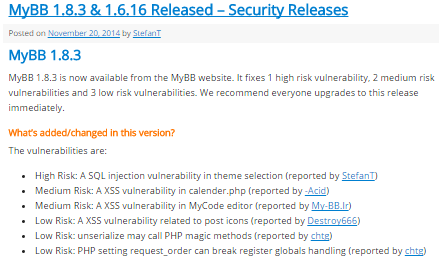
\includegraphics[scale=0.5]{figures/screen1}
      \end{figure}
    \end{column}
  \end{columns}
\end{frame}

\begin{frame}{Platforma}
  \begin{columns}
    \begin{column}[c]{0.50\textwidth}
      \begin{figure}
        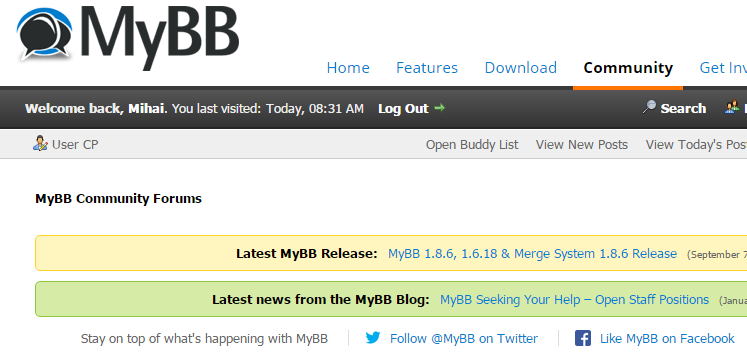
\includegraphics[scale=0.3]{figures/screen2}
      \end{figure}
    \end{column}
    \begin{column}[c]{0.50\textwidth}
        \begin{itemize}
		\vskip10pt
		\item \textbf{Front End} \& \textbf{Back End}(Admin CP)
		\vskip10pt
		\item structură ierarhizată a directoarelor
		\vskip10pt
		\item obscurity
		\vskip10pt
		\item levele diferite de autentificare \& permisiuni
	\end{itemize}
    \end{column}
  \end{columns}
\end{frame}

\begin{frame}{Înregistrare / Autentificare}
  \begin{columns}
    \begin{column}[c]{0.50\textwidth}
      \begin{figure}
        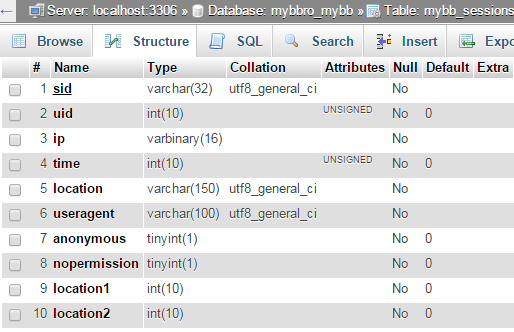
\includegraphics[scale=0.4]{figures/screen3}
      \end{figure}
    \end{column}
    \begin{column}[c]{0.50\textwidth}
        \begin{itemize}
		\vskip10pt
		\item autentificare pe bază de credențiale
		\vskip10pt
		\item restricții privind complexitatea parolei
		\vskip10pt
		\item mecanism de sesiuni + cookie-uri
		\vskip10pt
		\item failed logins, human detection
	    \end{itemize}
    \end{column}
  \end{columns}
\end{frame}

\begin{frame}{Statutul de membru}
  \begin{columns}
    \begin{column}[c]{0.50\textwidth}
        \begin{itemize}
		\vskip10pt
		\item asignat unui grup
		\vskip10pt
		\item super administrator
		\vskip10pt
		\item input-ul său este filtrat
		\vskip10pt
		\item jurnalizarea tuturor acțiunilor sale
	    \end{itemize}
    \end{column}
    \begin{column}[c]{0.50\textwidth}
      \begin{figure}
        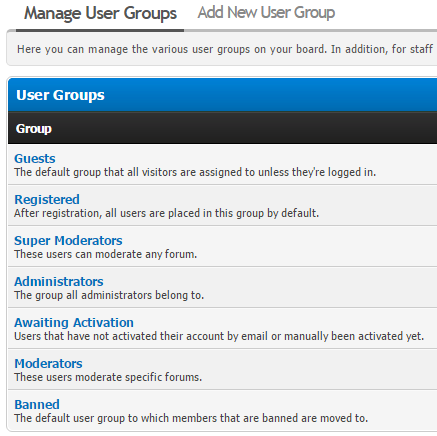
\includegraphics[scale=0.4]{figures/screen4}
      \end{figure}
    \end{column}
  \end{columns}
\end{frame}

\section[]{Posibile îmbunătățiri}

\begin{frame}{Posibile îmbunătățiri (I)}
\begin{itemize}
    \item \Large{TODO}
    \begin{itemize}
		\vskip5pt
		\item TODO
		\vskip5pt
		\item TODO
	\end{itemize}
	\vskip10pt
	\item \Large{TODO}
    \begin{itemize}
		\vskip5pt
		\item TODO
		\vskip5pt
		\item TODO
	\end{itemize}
	\item \Large{TODO}
    \begin{itemize}
		\vskip5pt
		\item TODO
		\vskip5pt
		\item TODO
	\end{itemize}
\end{itemize}
\end{frame}

\begin{frame}{Posibile îmbunătățiri (II)}
\begin{itemize}
    \item \Large{TODO}
    \begin{itemize}
		\vskip5pt
		\item TODO
		\vskip5pt
		\item TODO
	\end{itemize}
	\vskip10pt
	\item \Large{TODO}
    \begin{itemize}
		\vskip5pt
		\item TODO
		\vskip5pt
		\item TODO
	\end{itemize}
	\item \Large{TODO}
    \begin{itemize}
		\vskip5pt
		\item TODO
		\vskip5pt
		\item TODO
	\end{itemize}
\end{itemize}
\end{frame}

\section[]{Concluzii}

\begin{frame}{Concluzii}
	\begin{itemize}
	    \item TODO
	    \vskip10pt
	    \item TODO
	    \vskip10pt
	    \item TODO
    \end{itemize}
\end{frame}

\begin{frame}{Referințe \& Întrebări}
  \begin{columns}
    \begin{column}[c]{0.70\textwidth}
        \begin{thebibliography}{10}    
        \beamertemplatebookbibitems
            \bibitem{Reference1}
            MyBB Team
            \newblock {\em Security Research}
            \newblock January 2016
        \beamertemplatearticlebibitems
            \bibitem{Reference2}
            MyBB Team
            \newblock {\em Protecting Your MyBB Forum}
            \newblock January 2016
        \beamertemplatearticlebibitems
            \bibitem{Reference3}
            Nathan Malcolm
            \newblock {\em Multiple Security Tutorials}
            \newblock 2013-2015
        \beamertemplatearticlebibitems
            \bibitem{Reference4}
            Dingjie Yang
            \newblock {\em How a Missing Security Check Enabled a CSRF Attack}
            \newblock February 2015
        \end{thebibliography}
    \end{column}

    \begin{column}[c]{0.30\textwidth}
      \begin{figure}
        
\includegraphics[scale=0.2]{figures/question}
      \end{figure}
    \end{column}
  \end{columns}
\end{frame}

\end{document}